\documentclass[mathserif, 10pt]{beamer}
\usepackage[utf8]{inputenc}
\usepackage{amsmath, amsfonts}
\usepackage{appendixnumberbeamer}


\title[A Glance into Flavour Physics...]{A Glance into Flavour Physics \\with Effective Field Theories\\ and Machine Learning}
\author[Jorge Alda]{Jorge Alda,\\ Universidad de Zaragoza/CAPA\\
Università degli Studi di Padova/INFN \hspace{2em} \texttt{jalda@unizar.es} }

\date[PhD Thesis]{28th April 2022}



\usetheme{Zaragoza}
\usecolortheme{Unizar}
\titlepagelogoA{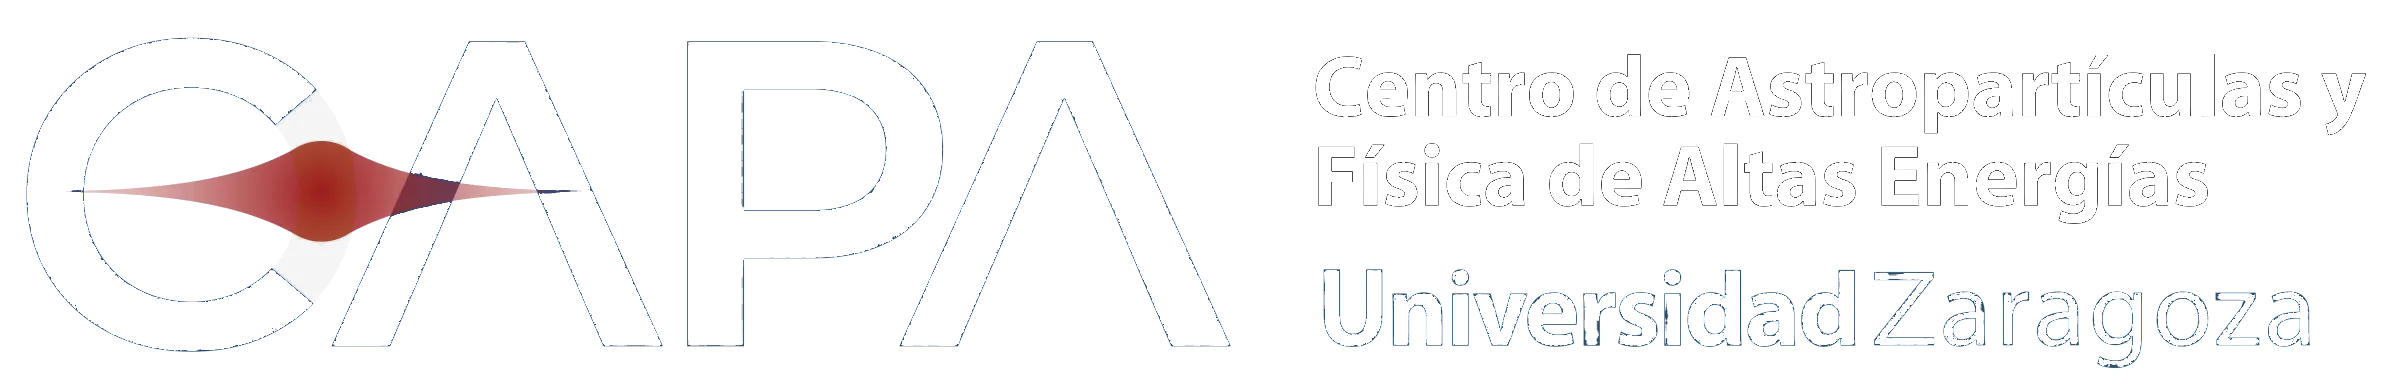
\includegraphics[width=6cm]{logos/CAPA.png}}
\titlepagelogoB{
\includegraphics[width=4cm]{logos/dftuz2.png}}


\newcommand\colorcite[1]{{\scriptsize\color{blue}#1}}

\begin{document}
\begin{frame}[noframenumbering,plain]

\titlepage

\end{frame}

\begin{frame}\frametitle{Publication List}

    \begin{itemize}
        \item J. Alda, J. Guasch, S. Peñaranda,
              \textit{Some Results on Lepton Flavour Universality Violations,}\\
              Eur. Phys. J. C 79.7 (2019), p.588, arXiv:1805.03636 [hep-ph].
        \item J. Alda, J. Guasch, S. Peñaranda, \textit{Anomalies in B meson decays: A phenomenological approach,}\\
              Eur. Phys. J. Plus 137 (2022), p.217, arXiv: 2012.14799 [hep-ph].
        \item J. Alda, J. Guasch, S. Peñaranda,
              \textit{Using Machine Learning techniques in phenomenological studies in flavour physics,}\\
              arXiv:2109.07405 [hep-ph].
        \item J. Alda, A. W. M. Guerrera, S. Peñaranda, S. Rigolin,
              \textit{Leptonic Meson Decays into invisible ALP,}\\
              arXiv:2111.02536 [hep-ph].
    \end{itemize}

\end{frame}

\begin{frame}
    \frametitle{Part I: $B$ physics}
\end{frame}

\begin{frame}\frametitle{$B$ anomalies}

    Flavour-changing neutral currents $b \to s \ell^+ \ell^-$, with $\ell = e, \mu$.
    \begin{itemize}
        \item Universality ratios $R_{K^{(*)}}$
              $$R_{K^{(*)}} = \frac{\mathrm{BR}(B\to K^{(*)}\mu^+ \mu^-)}{\mathrm{BR}(B\to K^{(*)}e^+ e^-)}\,, $$
              In the SM, theoretically clean, and $R_{K^{(*)}}=1$.\\
              LHCb measurements\footnote{R. Aaij \textit{et al.} (LHCb) arXiv:2103.11769, arXiv:1705.05802}:
              \begin{itemize}
                  \item $R_{K^+} = 0.846^{+0.042}_{-0.039}{}^{+0.013}_{-0.012}$,
                  \item $R_{K^{*0}} = 0.685^{+0.113}_{-0.069}\pm0.047$. ($3.1\,\sigma$ tension)
              \end{itemize}
        \item Angular observables for $B\to K^* \ell^+\ell^-$: $P'_4$, $P'_5\ldots$
        \item Also $B_s \to \phi \mu^+ \mu^-$ decays.
    \end{itemize}

\end{frame}

\begin{frame}\frametitle{$B$ anomalies}
    Flavour-changing charged currents $b\to c \ell \nu$, with $\ell = e/\mu, \tau$.
    \begin{columns}
        \begin{column}{0.55\textwidth}

            \begin{itemize}
                \item Universality ratios $R_{D^{(*)}}$
                      $$R_{D^{(*)}} = \frac{\mathrm{BR}(B\to D^{(*)}\tau \nu)}{\mathrm{BR}(B\to D^{(*)}\ell \nu)}\,, $$
                      $$R_D = 0.340 \pm 0.027 \pm 0.013\,,$$
                      $$R_{D^*} = 0.295 \pm 0.011 \pm 0.008\,.$$
                      Combined tension of $3.08\,\sigma$.\footnotemark[1]
                \item Longitudinal polarization of $D^*$.
                \item Also $B_c \to J/\psi \ell\nu$ decays.
            \end{itemize}

        \end{column}
        \begin{column}{0.5\textwidth}
            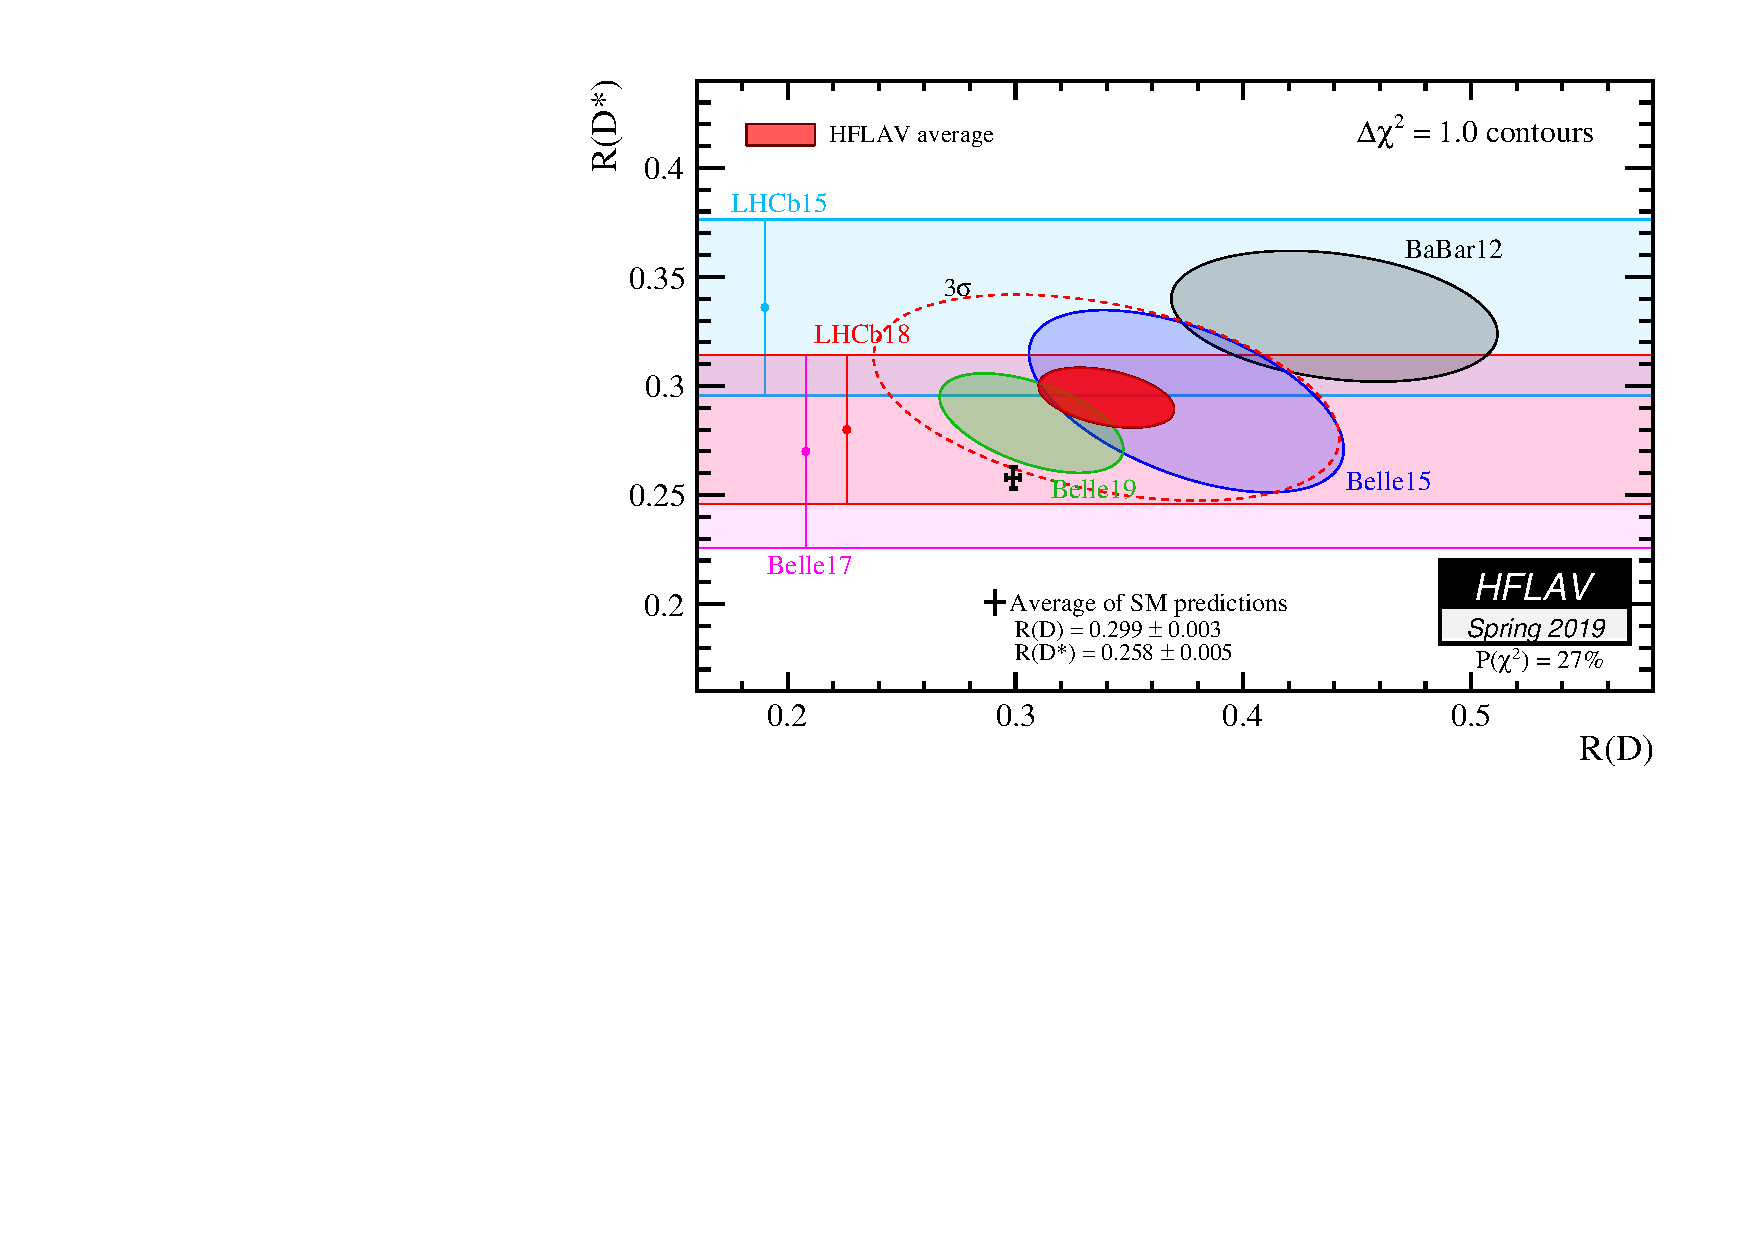
\includegraphics[width=\columnwidth]{figures/rdrds_spring2019.pdf}
        \end{column}
    \end{columns}
    \footnotetext[1]{Y. S. Ahmis \textit{et al.} (HFLAV) arXiv:1909.12524}
\end{frame}

\begin{frame}\frametitle{Effective Field Theory}
    \setbeamercovered{transparent}
    \def\beamertemplatetransparentcoveredmedium{\setbeamercovered{transparent=50}}
    \beamertemplatetransparentcoveredmedium
    \begin{itemize}
        \item  EFT ``integrates out" heavy degrees of freedom above energy scale $\Lambda$, resulting in operators with dim $> 4$. The short-distance physics is encoded in the Wilson coefficient that multiplies each operator.
              $$\mathcal{L}_\mathrm{EFT} = \mathcal{L}_\mathrm{SM} + \frac{1}{\Lambda}\sum C^{(5)} \mathcal{O}^{(5)} + \frac{1}{\Lambda^2}\sum C^{(6)} \mathcal{O}^{(6)} + \cdots$$
              \vspace{-2mm}
        \item In particular, SMEFT integrates out all NP degrees of freedom.
              \begin{itemize}
                  \item Model-independent description.
                  \item 2499 dimension-6 operators ($\Delta B = \Delta L = 0$).
                  \item Warsaw basis\footnotemark[2] is the most common choice.
                  \item We will consider NP contributions to the following operators:
                        $$\mathcal{O}_{\ell q(1)}^{ijkl} = (\bar{\ell}_i \gamma_\mu \ell_j)(\bar{q}_k \gamma^\mu  q_l), \qquad \mathcal{O}_{\ell q(3)}^{ijkl} = (\bar{\ell}_i \gamma_\mu \tau^I \ell_j)(\bar{q}_k \gamma^\mu \tau^I q_l).$$
                        \footnotetext[2]{Grzadkowski, M. Iskrzynski, M. Misiak, J. Rosiek,    JHEP 10 (2010) 085. arXiv:1008.4884}
              \end{itemize}
    \end{itemize}
\end{frame}

\begin{frame}\frametitle{Effective Field Theory}
\begin{itemize}

\item The scale of $B$ decays is $\mu \approx m_b$. We need to integrate out $t$, $H$, $W$ and $Z$.

\item The Weak Effective Theory (WET) Lagrangian is given by
{\scriptsize $$\mathcal{L}_{\text{WET}} = \mathcal{L}_\mathrm{SM} -\frac{4 G_F}{\sqrt{2}}V_{cb}\sum_{\ell = e, \mu, \tau} (1 + C_{VL}^\ell) \mathcal{O}_{VL}^\ell + \frac{4G_F}{\sqrt{2}}V_{tb}V_{ts}^*\frac{e^2}{16\pi^2}\sum_{\ell=e,\mu} (C_9^\ell \mathcal{O}_9^\ell  + C_{10}^\ell \mathcal{O}_{10}^\ell) \ ,$$}
{ $$\mathcal{O}_{VL}^\ell = (\bar{c}_L \gamma_\alpha b_L)(\bar{\ell}_L \gamma^\alpha \nu_\ell)\ ,$$ $$\mathcal{O}_9^\ell = (\bar{s}_L \gamma_\alpha b_L)(\bar{\ell} \gamma^\alpha \ell)\ , \qquad \mathcal{O}_{10}^\ell = (\bar{s}_L \gamma_\alpha b_L)(\bar{\ell} \gamma^\alpha \gamma_5 \ell) \ .$$}
    
\item To relate the Wilson coefficients at both scales:
\begin{enumerate}
    \item Run the SMEFT RG equations from $\Lambda$ down to EW scale.
    \item Match the SMEFT operators to the WET operators.
    \item Run the WET RG equations from EW scale down to $m_b$.
\end{enumerate}
    
\end{itemize}
\end{frame}

\end{document}